Determinističko križanje (\textit{eng. deterministic functional crossover}), opisano u \cite{crxDeter}, ostvaruje križanje dvije jedinke na osnovi funkcijske sličnosti. Ovaj operator primjenjiv je samo na probleme simboličke regresije.

Kako bi se funkcijska sličnost dva gena, odnosno čvorova stabla koji izgrađuju jedinku, mogla odrediti, za svaki gen zapisuje se minimalna i maksimalna vrijednost koju može poprimiti za podatke iz skupa za učenje. Funkcijska sličnost (u radu nazvana funkcijskom udaljenošću) između dva gena i i j, računa se kao:

\begin{equation} 
\label{udaljenost}
 \large{ d_{i,j} = \frac{1}{2} (|max_i - max_j| + |min_i - min_j|) }
\end{equation}
\\
U radu je opisan glavni nedostatak ovog križanja - postoji velika vjerojatnost da križanje koje se dogodi pod utjecajem ovog operatora bude neutralno, odnosno, da se novonastala jedinka uopće ne razlikuje od jednog od roditelja. Ovaj slučaj dogodi se kada se u prvom roditelju izabere podstablo koje je strukturno jednako odabranom podstablu drugog roditelja (može biti interpretirano na jednak način nakon što se izraz predstavljen podstablom simplificira). Križanjem takvih podstabala, originalno ponašanje se uopće ne mijenja te je rezultantna jedinka potpuno jednaka svome roditelju. Pojava neutralnog križanja to je češća što jedinke sve više i više rastu (čime se povećava vjerojatnost odabira strukturno jednakog podstabla). Kako bi se riješio ovaj problem, u istom radu predloženo je probabilističko križanje, koje je opisano u idućem poglavlju.

\subsection{Dosadašnji rezultati}
Na slici \ref{deto} prikazani su grafovi usporedbe učinkovitost determinističkog križanja u usporedbi s jednostavnim i probabilističkim križanjem i slučaja kada nije upotrijebljen niti jedan operator križanja. Pri tome, grafovi na lijevoj strani pokazuju performanse dobivenih rješenja na skupu za učenje, a oni na desnoj strani, performanse na skupu za testiranje. Eksperimenti su bili provedeni na primjerima simboličke regresije. Na desnoj strani slike, vidljivo je kako ne postoji prevelika razlika između učinkovitosti danih operatora. 


\begin{figure}[H]
	\centering
	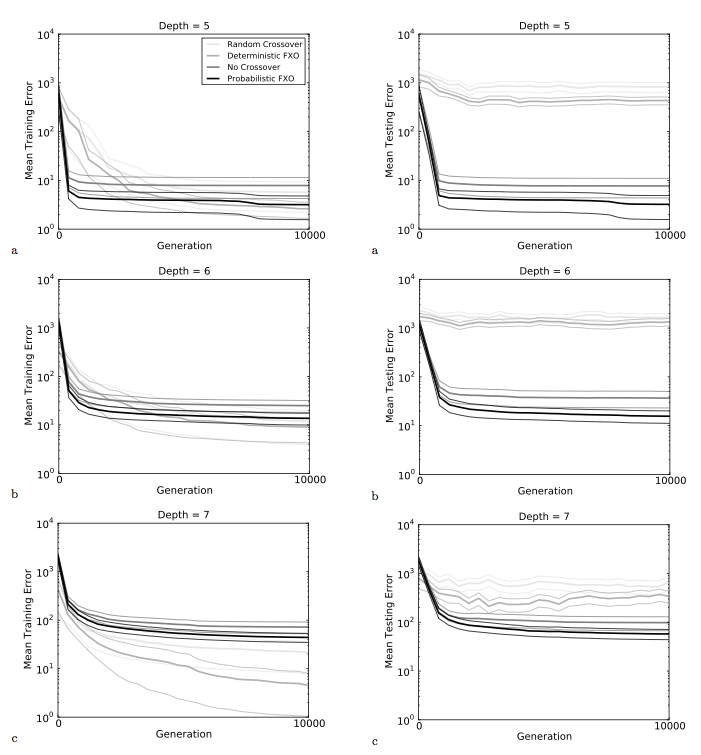
\includegraphics[scale=0.65]{./slike/deto.png}
	\caption{Usporedba učinkovitosti determinističkog, jednostavnog i probabilističkog križanja i slučaja kada nije upotrijebljen niti jedan operator križanja}
	\label{deto}
\end{figure}

Također, vidljivo je kako je ovo križanje dalo superiorno rješenje na skupu za učenje naspram ostalima za slučaj kada je dubina stabla jednaka 7. U suprotnosti, odnosno, posljedično tome, na skupu za testiranje isti slučaj dao je značajno slabije rezultate što upućuje na prenaučavanje jedinki.

Također, pokazano je da ovo križanje ne podržava prekomjeran rast jedinki tijekom generacije. Dapače, dana rješenja često su ispala nešto manja od onog ciljanog.




\section{Probabilističko križanje}

Kako bi se riješio problem neutralnog križanja koji se pojavio kod determinističkog križanja, u \cite{crxDeter} je predloženo probabilističko križanje (eng. probabilistic functional crossover). Jednako kao i kod determinističkog križanja, za svaki čvor u stablu zapisuje se minimalna i maksimalna vrijednost čvora za podatke iz skupa za učenje (izraz \ref{udaljenost}).

Prilikom križanja, nakon što se u prvom stablu nasumično odabere točka križanja izračunava se funkcionalna udaljenost između njega i svakog čvora unutar drugog roditelja (jednako kao i kod determinističkog križanja). Nakon što su dobivene sve moguće udaljenosti, one se normaliziraju prema \ref{norm}:

\begin{equation} 
\label{norm}
 \large{ d '_{i,j} = \frac{d_{i,j}}{\sum_{k=1}^{s} d_{i,k}} }
\end{equation}
 
Normalizacija je pogodna iz razloga što se s najvećom vjerojatnošću želi odabrati funkcionalno najbliži čvor. Ovako dobivene normalizirane udaljenosti potom se invertiraju i ponovno normaliziraju u odnosne na te invertirane vrijednosti prema \ref{prob}:
 
 \begin{equation} 
\label{prob}
 \large{ p_{i,j} = \frac{1 - d '_{i,j}}{\sum_{k=1}^{s} (1 - d '_{i,k})} }
\end{equation}

Time dobivamo to veću vjerojatnost što je udaljenost između dva čvora manja. Nakon ovih operacija, nasumično, ali s izračunatim vjerojatnostima, odabire se podstablo unutar drugog roditelja koje će se iskoristiti za križanje. Pokazano je kako ovakvo križanje pridonosi većem postotku korisnog križanja, a time i bržoj konvergenciji nego uobičajeni operatori, iako je priznato kako je ovakav izračun udaljenosti prilično gruba aproksimacija funkcionalne udaljenosti.

\subsection{Dosadašnji rezultati}
Jednako kao i za determinističko križanje, provedeni eksperimenti za ovo križanje uključuju usporedbu probabilističkog, determinističkog i jednostavnog križanja i slučaja kada nije upotrijebljen niti jedan operator križanja. Rezultati su prikazani su na slici \ref{deto}. Vidljivo je kako probabilističko križanje konstantno bolje djeluje od jednostavnog križanja i slučaja kada se ne koristi niti jedan operator križanja.

Osim toga, dokazano je kako je korisnost križanja \footnote{križanje se smatra korisnim ukoliko producira jedinku koja ima dobrotu bolju od oba roditelja}, kada se koristi probabilistički operator križanja, puno veća nego u ostalim slučajevima. Pokazano je kako se ovim križanjem dobivaju jedinke koje su značajno veće od točnog rješenja. Naravno, pitanje je kako interpretirati ovu pojavu, budući da se izraz koji predstavlja jedinka gotovo uvijek može pojednostavniti čime bi stablo bilo puno manje.

Uočena je korelacija između veličine roditelja i događanja korisnog križanja. No, to je i za očekivati iz razloga što je omjer broja listova na prema unutarnjim čvorovima to veći što je samo stablo veće. Radi toga, vjerojatnost odabira lista za ulazak u križanje se povećava, čime se i smanjuje mogućnost za destruktivnim križanjem. 